\documentclass[12pt]{lab}
\graphicspath{{pics/}}
\DeclareGraphicsExtensions{.pdf,.png,.jpg,.eps}
\pagestyle{fancy}
\usepackage{unicode}
\usepackage{multicol}
\usepackage{multirow}
\usepackage{tikz}

\title {Лабораторная работа 3.4.5}
\author{Сидорчук Максим, Б01-304}
\date{\today}

\begin{document}
\maketitle

\paragraph*{Цель работы:} изучение петель гистерезиса ферромагнитных
материалов с помощью осциллографа.

\paragraph*{Оборудование:} автотрансформатор, понижающий
трансформатор, амперметр и вольтметр (мультиметры), резистор,
делитель напряжения, интегрирующая
цепочка, электронный осциллогра, тороидальные образцы с двумя обмотками..

\section{Теоретическое введение}

\begin{wrapfigure}{l}{0.6\textwidth}
    \vspace{-20pt}
    \begin{center}
        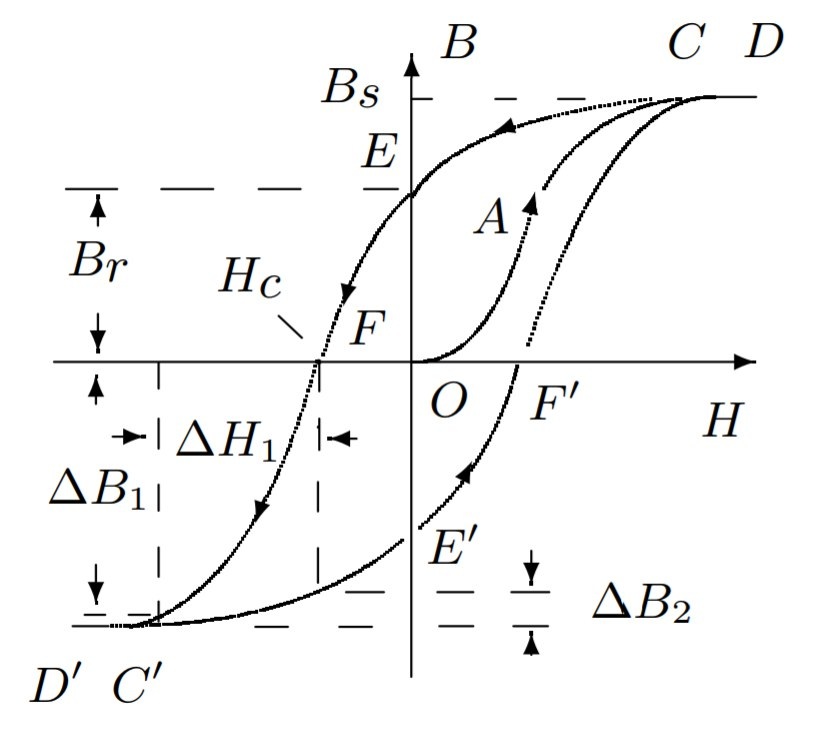
\includegraphics[width=0.7\linewidth]{gist3.jpg}
        \label{fig:sdfsafd}
    \end{center}
    \vspace{-10pt}
    \caption{Петля гистерезиса ферромагнетика}
\end{wrapfigure}

Магнитная индукция $\vec{B}$ и напряженность магнитного поля
$\vec{H}$ в ферромагнитном материале неоднозначно связаны
между собой: индукция зависит не только от напряженности, но
и от предыстории образца. Связь между индукцией
и напряженностью поля типичного ферромагнетика иллюстрирует рис. 1. Если
к размагниченному образцу начинают прикладывать магнитное поле, то
его намагничивание следует кривой $ OACD $, выходящей
из начала
координат. Эту кривую называют \textit{основной кривой намагничивания}.

Индукция $\vec{B}$ в образце состоит из индукции, связанной с
намагничивающим полем
$\vec{B}$, и индукции, создаваемой самим намагниченным
образцом.
В системе СИ эта связь имеет вид

$$\vec{B} = \mu_{0}(\vec{H}+\vec{M}),$$

где $\vec{M}$- \textit{намагниченность} - магнитный момент единичного
объема образца, а $\mu_{0}$ - магнитная постоянная.

Намагнитим образец до насыщения - до точки D. Соответствующее
значение индукции $B_{s}$ называют индукцией насыщения. При
уменьшении поля $H$ до нуля зависимость $B(H)$ имеет вид кривой
$DCE$, и при нулевом поле индукция имеет конечное ненулевое значение.
Это остаточная индукция $B_{r}$ . Чтобы размагнитить образец, то есть
перевести его в состояние
$F$, необходимо приложить "обратное" магнитное
поле $H_{c}$, которое называют коэрцитивной силой.

Замкнутая кривая $DEFD'E'F'D'$, возникающая при циклическом
перемагничивании образца, намагниченного до насыщения, называется
\textit{предельной петлей гистерезиса.}

\subsection{Измерение магнитной индукции в образцах.}
Магнитную индукцию удобно определять с помощью ЭДС, возникающей при
изменении магнитного потока Ф в катушке, намотанной на образец:

$$\mathscr{E} = -\dfrac{d\Phi}{dt}.$$

Тогда отсюда и из формулы $\Phi=BSN_{\text{и}}$ получаем:
$$|B|=\dfrac{1}{SN_{\text{и}}}\int \mathscr{E}dt.$$
Для интегрирования сигнала применяют интегрирующие схемы (рис. 2).

\begin{wrapfigure}{l}{0.6\textwidth}
    \vspace{-20pt}
    \begin{center}
        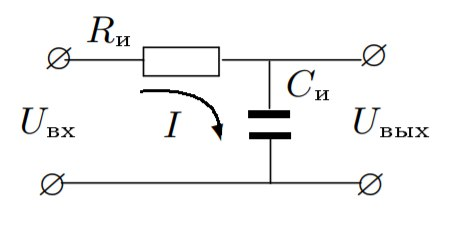
\includegraphics[width=0.7\linewidth]{gist2.jpg}
        \label{fig:}
    \end{center}
    \vspace{-10pt}
    \caption{Интегрирующая RC-цепь}
\end{wrapfigure}

Если выходной сигнал намного меньше входного ($U_\text{out}\ll U_\text{in},$)
ток в цепи пропорционален входному напряжению:
$I\simeq\dfrac{U_\text{in}}{R}$, а напряжение на емкости С

$$U_\text{out}\simeq\dfrac{1}{RC}\int U_\text{in}dt.$$

Этот вывод тем ближе к истине, чем больше постоянная $\tau=RC$
превосходит характерное время процесса (например, его период). Для
синусоидальных напряжений

$$U_\text{out}=\dfrac{U_\text{in}}{RC\Omega},$$

где $\Omega$ - частота сигнала.

В итоге, обозначив параметры интегрирующей цепи через $R_\text{и}$ и
$C_\text{и}$, получаем

$$ |B|=\dfrac{1}{SN_\text{и}}\int
U_\text{in}dt=\dfrac{R_\text{и}C_\text{и}}{SN_\text{и}}U_\text{out}.$$

\section{Экспериментальная установка.}
Схема экспериментальной установки показана на рис. 3.

Действующее значение переменного тока в обмотке N0 измеряется
амперметром А (мультиметром GDM). Последовательно с амперметром
включено сопротивление $R_{0}$, напряжение с которого подается на
вход X электронного осциллографа (ЭО). Это напряжение пропорционально
току в обмотке $N_{0}$, а следовательно и напряженности H магнитного
поля в образце.

Для измерения магнитной индукции B с измерительной обмотки $N_\text{И}$ на
вход интегрирующей RC -цепочки подается напряжение $U_\text{И}$ (UВХ),
пропорциональное производной $\dot{B}$, а с выхода снимается
напряжение $U_{C}$($U_\text{out}$), пропорциональное
величине B , и подается на вход Y осциллограа.
Замкнутая кривая, возникающая на экране, воспроизводит в некотором
масштабе (различном для осей X и Y ) петлю гистерезиса. Чтобы придать
этой кривой количественный смысл, необходимо установить масштабы
изображения, т.е. провести калибровку каналов X и Y ЭО. Для этого,
во-первых, надо узнать, каким напряжениям (или токам) соответствуют
амплитуды сигналов, видимых на экране, и во-вторых,  каким значениям
B и H соответствуют эти напряжения
(или токи).

\begin{figure}[H]
    \centering
    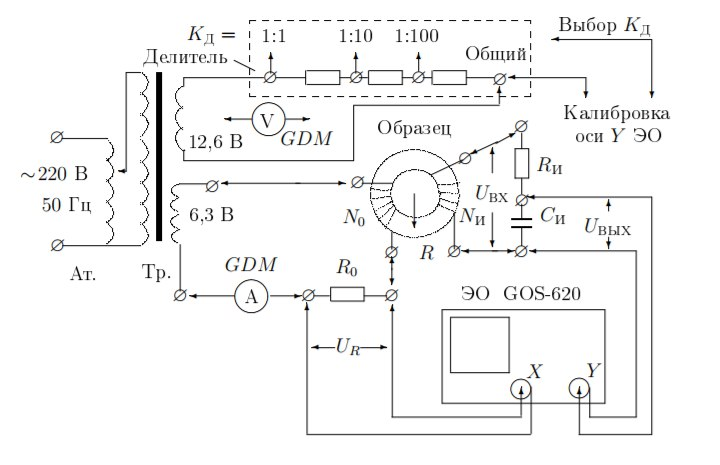
\includegraphics[width=\linewidth]{gist.jpg}
    \caption{Схема установки для исследования намагничивания образцов}
    \label{fig:Holl2}
\end{figure}

\section{Ход работы}

\begin{enumerate}
    \item Запишем данные установки:

        $R_{0}=1 \text{Ом} \ \ R_\text{и}=20 \text{кОм} \ \ C_\text{и}=20
        \text{мкФ} $

        Параметры тороидальных образцов:

        \begin{itemize}
            \item   \textbf{Кремниевое железо $ Fe-Si $}:
                $N_{0}=75$ витков;
                $N_\text{и}=400$ витков;
                $S=2.85 \text{см}^{2}$;
                $2\pi R = 11 \text{см} $.

            \item  \textbf{Пермаллой $ Fe-Ni $}:
                $N_{0}=40$ витков;
                $N_\text{и}=200$ витков;
                $S = 4.5 \text{см}^{2}$;
                $2\pi R = 14.1 \text{см} $.

            \item  \textbf{Феррит}:
                $N_{0}=85$ витков;
                $N_\text{и}=300$ витков;
                $S=3.0 \text{см}^{2}$;
                $2\pi R = 24 \text{см} $.
        \end{itemize}

    \item Соберем схему (рис. 3) и настроим оборудование.

    \item Для каждого образца сфотографируем предельную петлю.
        Запишем значения коэффициентов усиления $K_{x}$ и $K_{y}$,
        ток $I_\text{эф}$. Измерим двойные амплитуды для коэрцитивной силы
        $2x(c)$ и индукции насыщения $2y(s)$. Результаты таковы:

        \begin{itemize}
            \item   \textbf{Кремниевое железо}:

                $K_{x}=200 \dfrac{\text{мВ}}{\text{дел}},$
                $K_{y}=100 \dfrac{\text{мВ}}{\text{дел}},$
                $I_\text{эф}=1.03 \text{А}. $
                При этом $ 2x = 10.0 \text{дел}, \; 2y = 6.3 \text{дел}$.

                \begin{figure}[H]
                    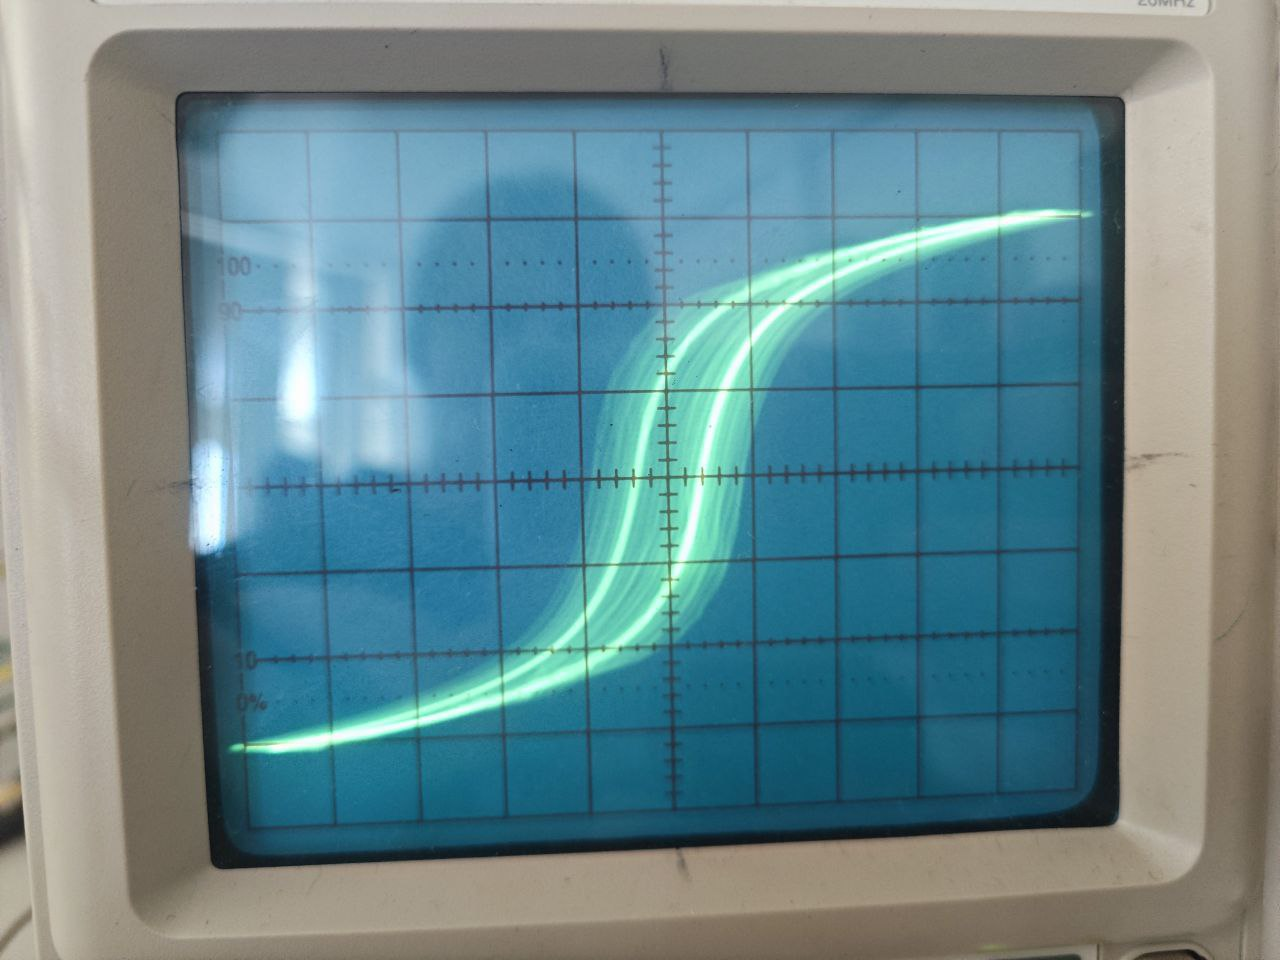
\includegraphics[width=\textwidth]{1.jpg}
                    \caption{Петля гистерезиса для кремниевого железа}
                \end{figure}

            \item   \textbf{Пермаллой}:

                $K_{x}=100 \dfrac{\text{мВ}}{\text{дел}},$
                $K_{y}=100 \dfrac{\text{мВ}}{\text{дел}},$
                $I_\text{эф}=218 \text{мА}. $
                При этом $ 2x = 7.6 \text{дел}, \; 2y = 4.0 \text{дел}$.

                \begin{figure}[H]
                    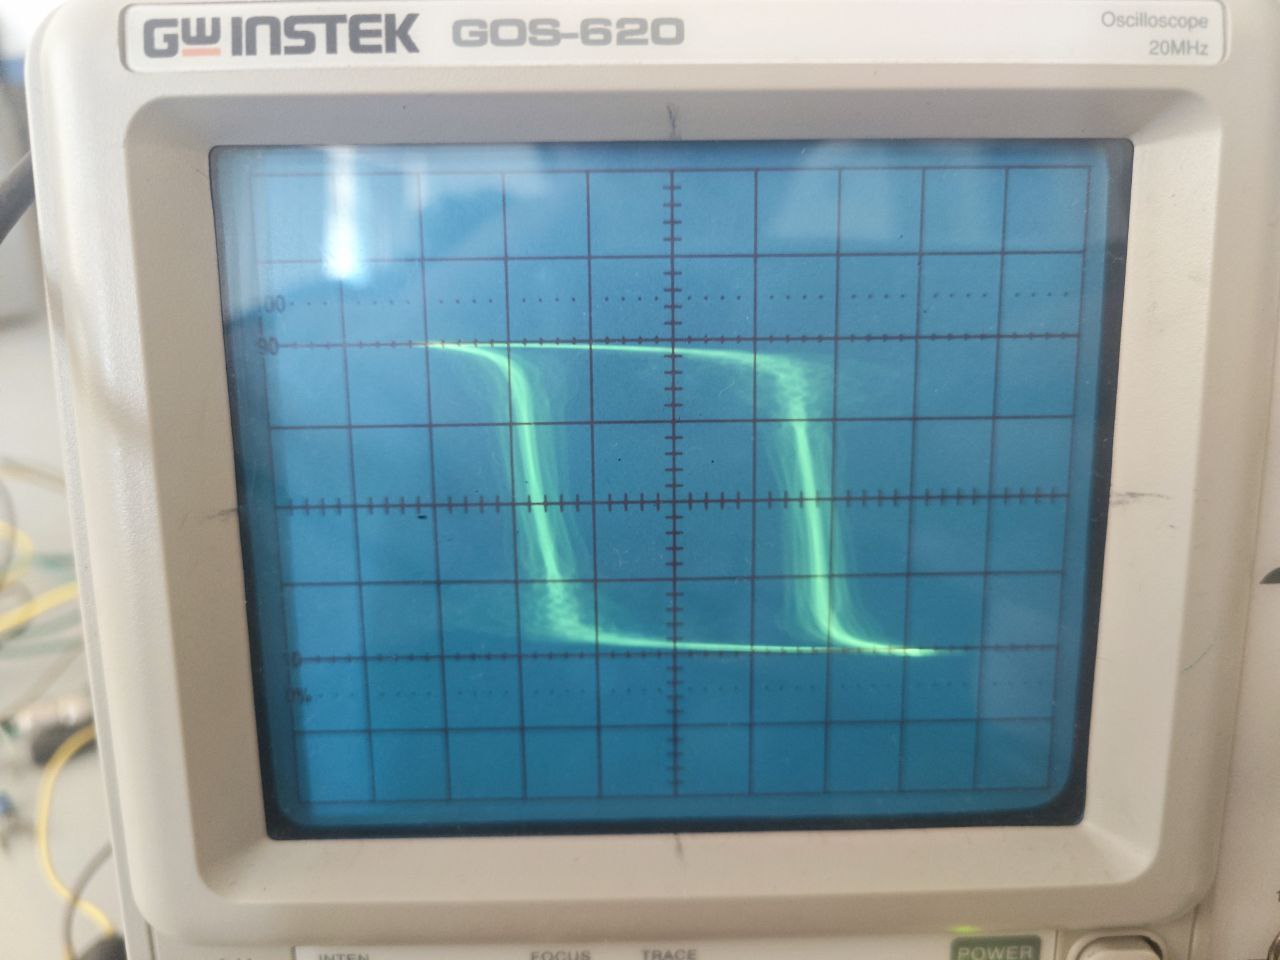
\includegraphics[width=\textwidth]{2.jpg}
                    \caption{Петля гистерезиса для пермаллоя}
                \end{figure}

            \item    \textbf{Феррит}:

                $K_{x}=500 \dfrac{\text{мВ}}{\text{дел}},$
                $K_{y}=50 \dfrac{\text{мВ}}{\text{дел}},$
                $I_\text{эф}=92.6 \text{мА}. $
                При этом $ 2x = 7.4 \text{дел}, \; 2y = 4.0 \text{дел}$.

                \begin{figure}[H]
                    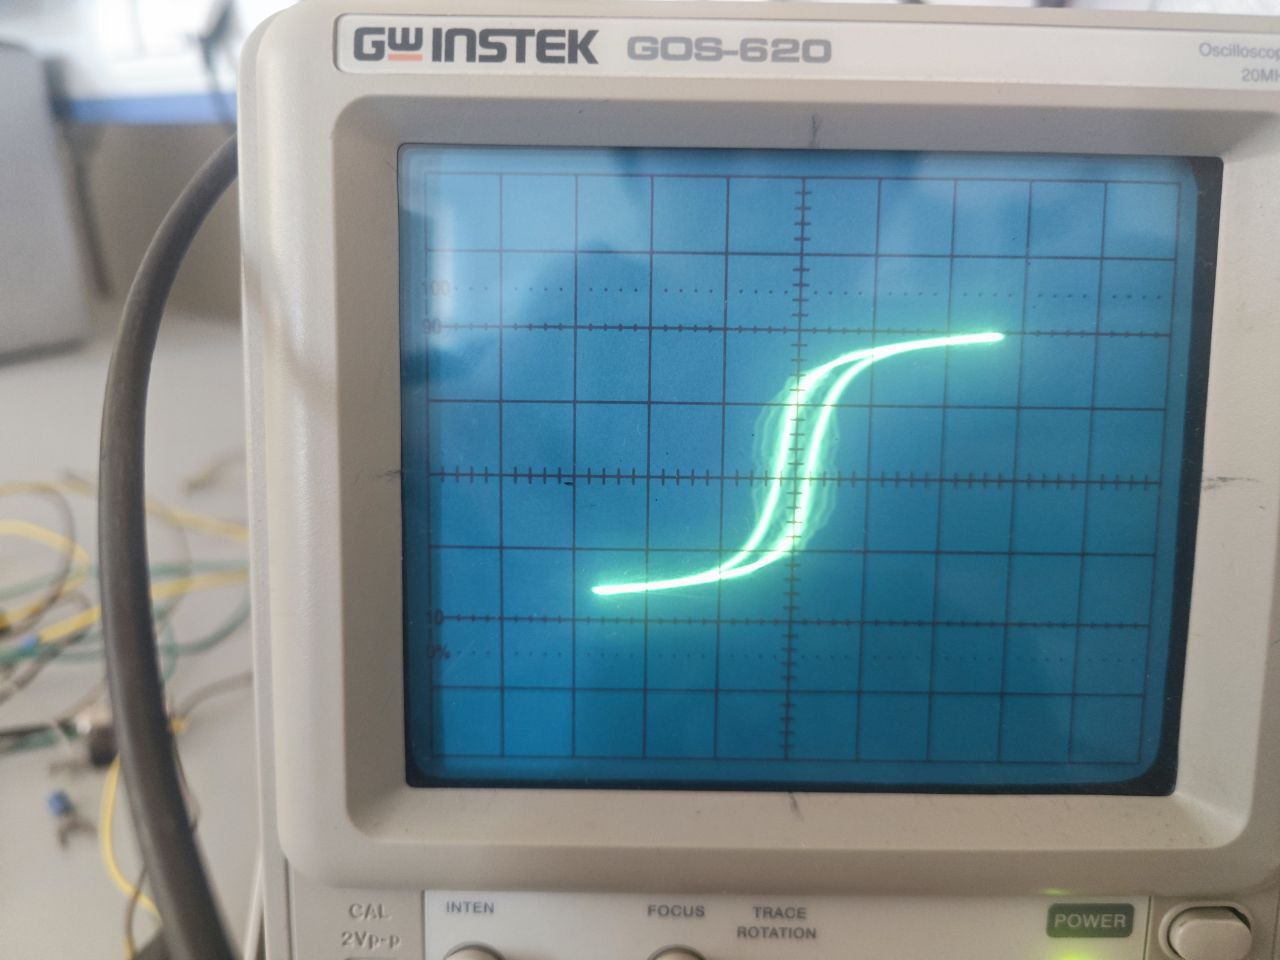
\includegraphics[width=\textwidth]{3.jpg}
                    \caption{Петля гистерезиса для феррита}
                \end{figure}

        \end{itemize}

    \item Снимем для каждого образца начальную кривую намагничивания
        (табл. 1-3), плавно уменьшая ток до нуля и отмечая вершины
        частных петель. По этим данным построим эти кривые (рис. 4-6).

        \begin{table}[H]
            \caption{Начальная кривая намагничивания кремнистого железа}
            \begin{center}
                \begin{tabular}{|c|*{15}{c|}}\hline
                    $ x $ & 5 & 4.4 & 4 & 3.5 & 3 & 2.5 & 2 & 1.5 & 1 & 0.8 & 0.6 & 0.4 & 0.2 & 0\\\hline
                    $ y $ & 3 & 2.9 & 2.8 & 2.7 & 2.6 & 2.5 & 2.4 & 2 & 1.6 & 1.4 & 1.2 & 0.8 & 0.2 & 0\\\hline
                \end{tabular}
            \end{center}
        \end{table}

        \begin{figure}[H]
            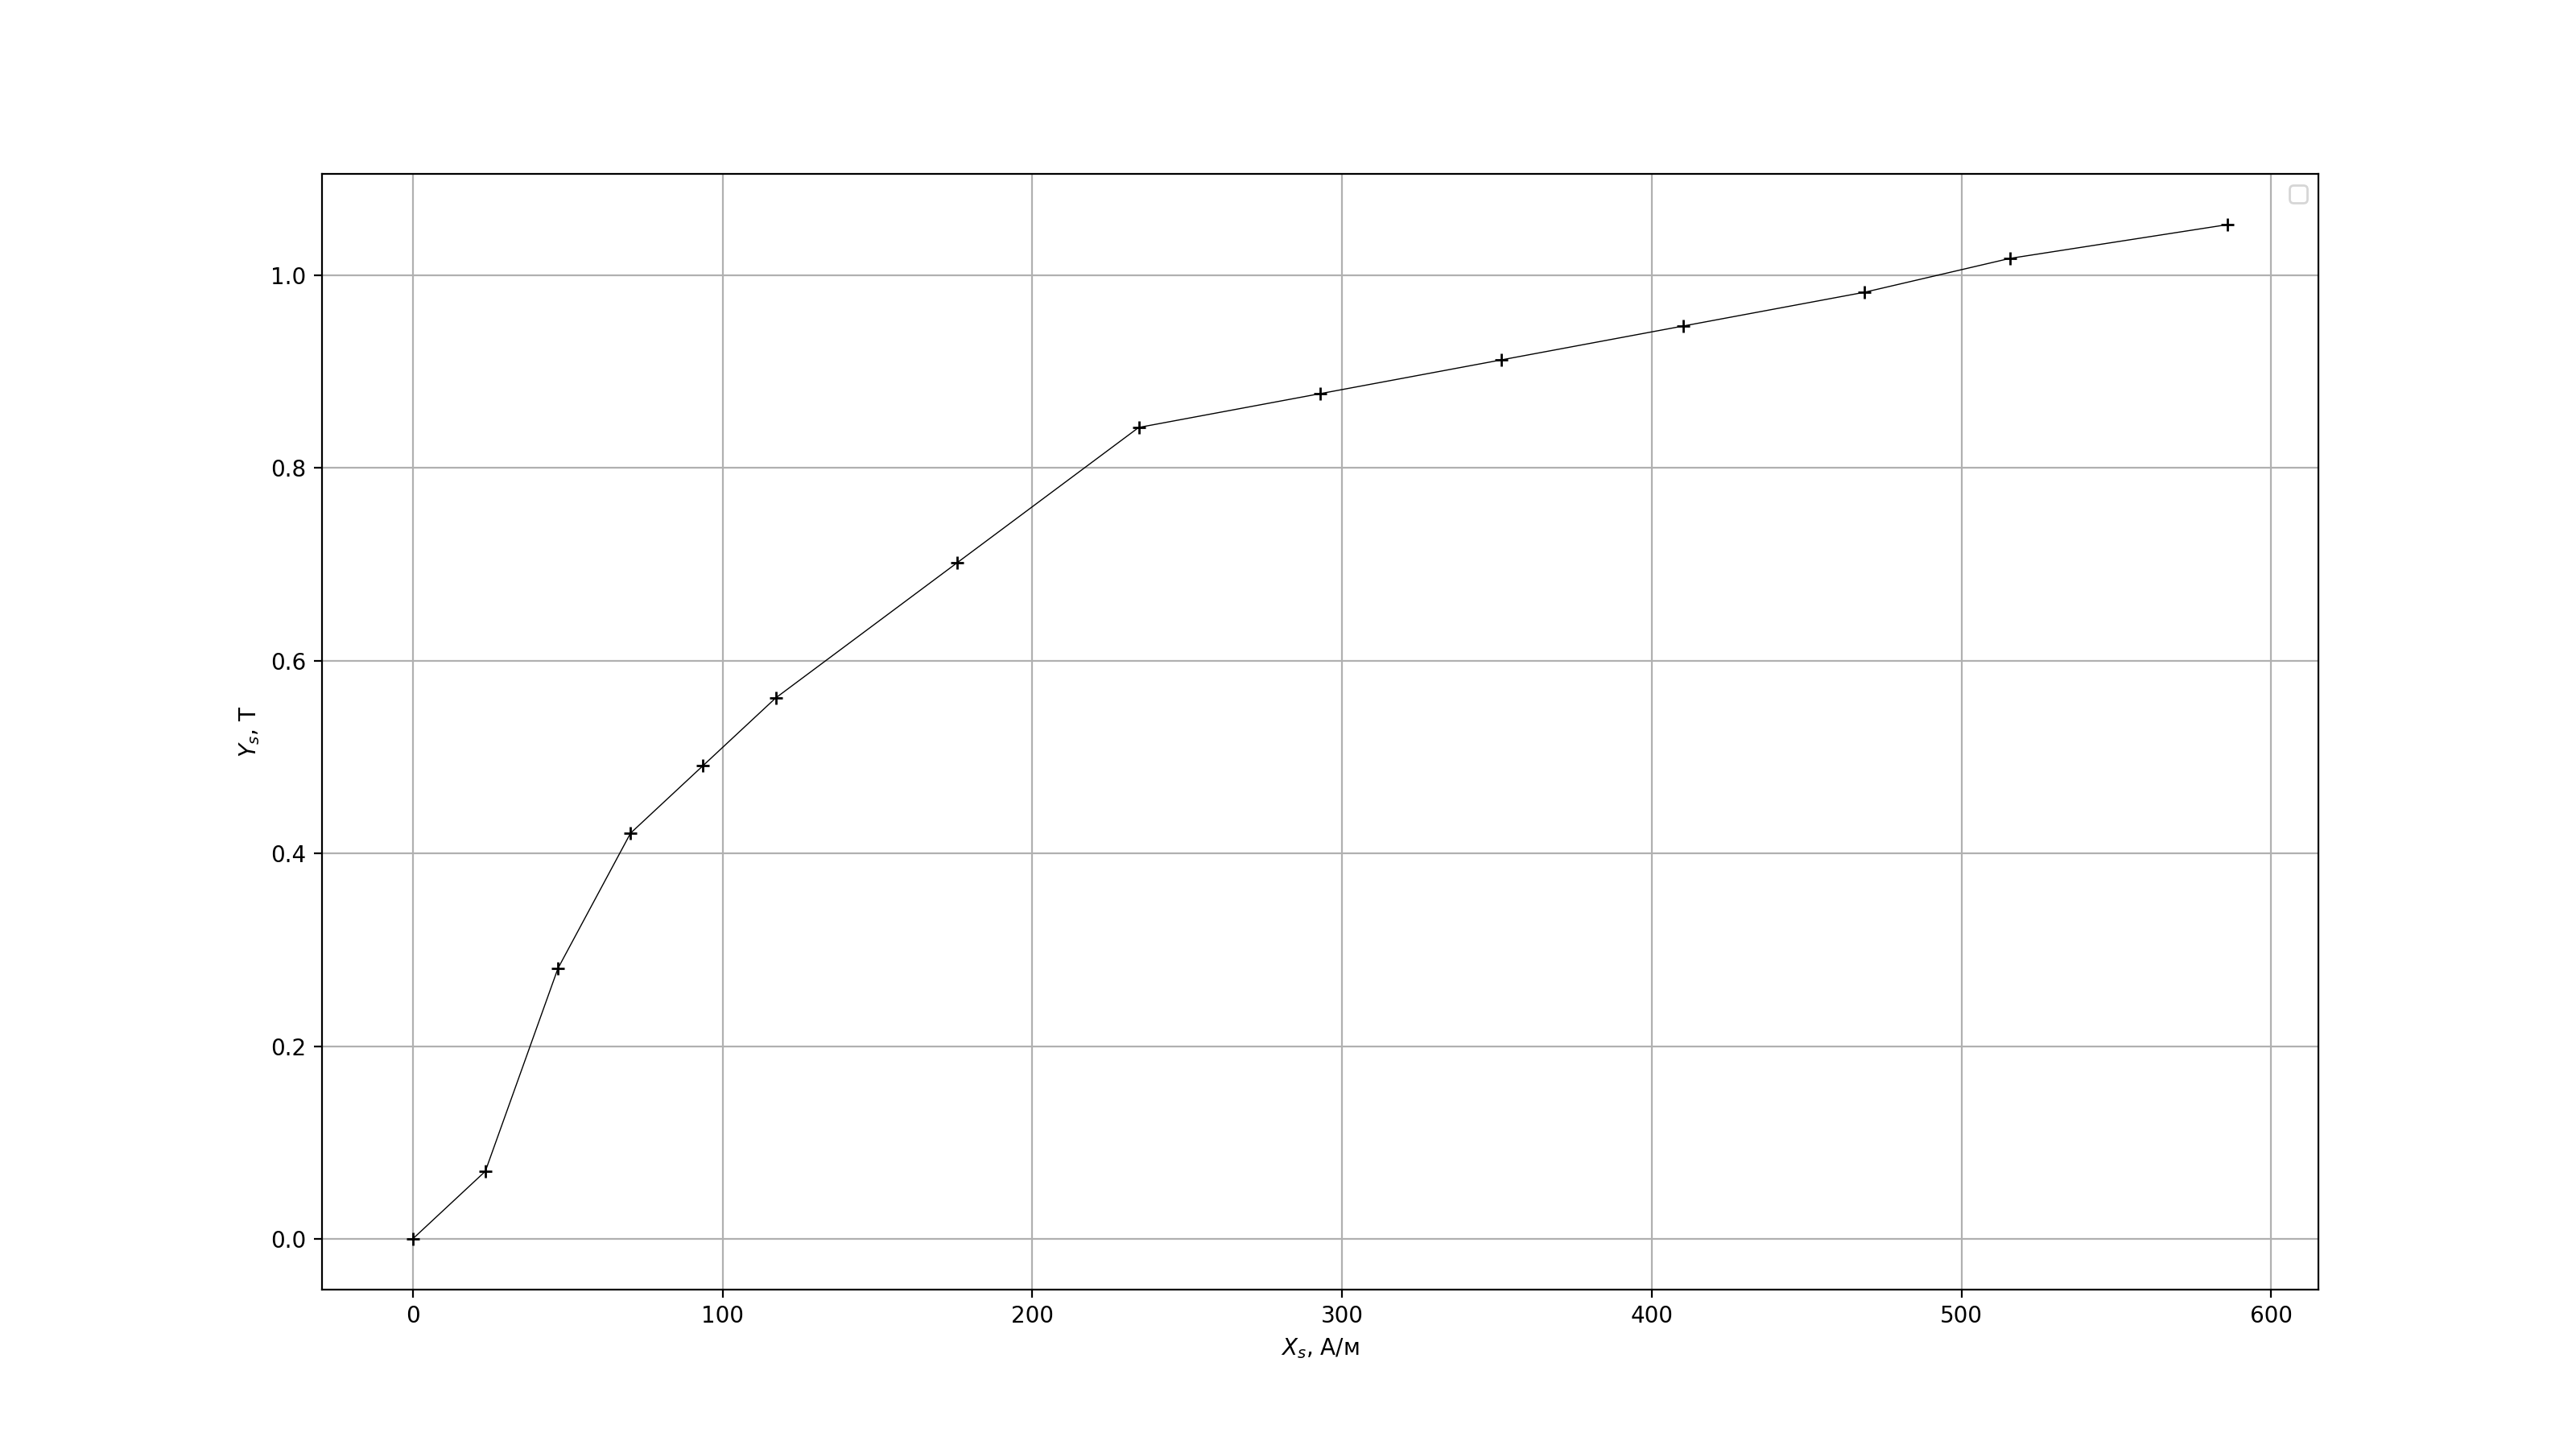
\includegraphics[width=\textwidth]{pics/graph1.png}
            \caption{Начальная кривая намагничивания кремнистого железа - график}
        \end{figure}

        \begin{table}[H]
            \caption{Начальная кривая намагничивания пермаллоя}
            \begin{center}
                \begin{tabular}{|c|*{15}{c|}}\hline
                    $x$ & 3 & 2.6 & 2 & 2 & 2 & 2 & 1.8 & 1.6 & 1.4 & 1.2 & 1\\\hline
                    $y$ & 2 & 1.9 & 1.8 & 1.4 & 1.2 & 1 & 0.8 & 0.6 & 0.4 & 0.2 & 0\\\hline
                \end{tabular}
            \end{center}
        \end{table}

        \begin{figure}[H]
            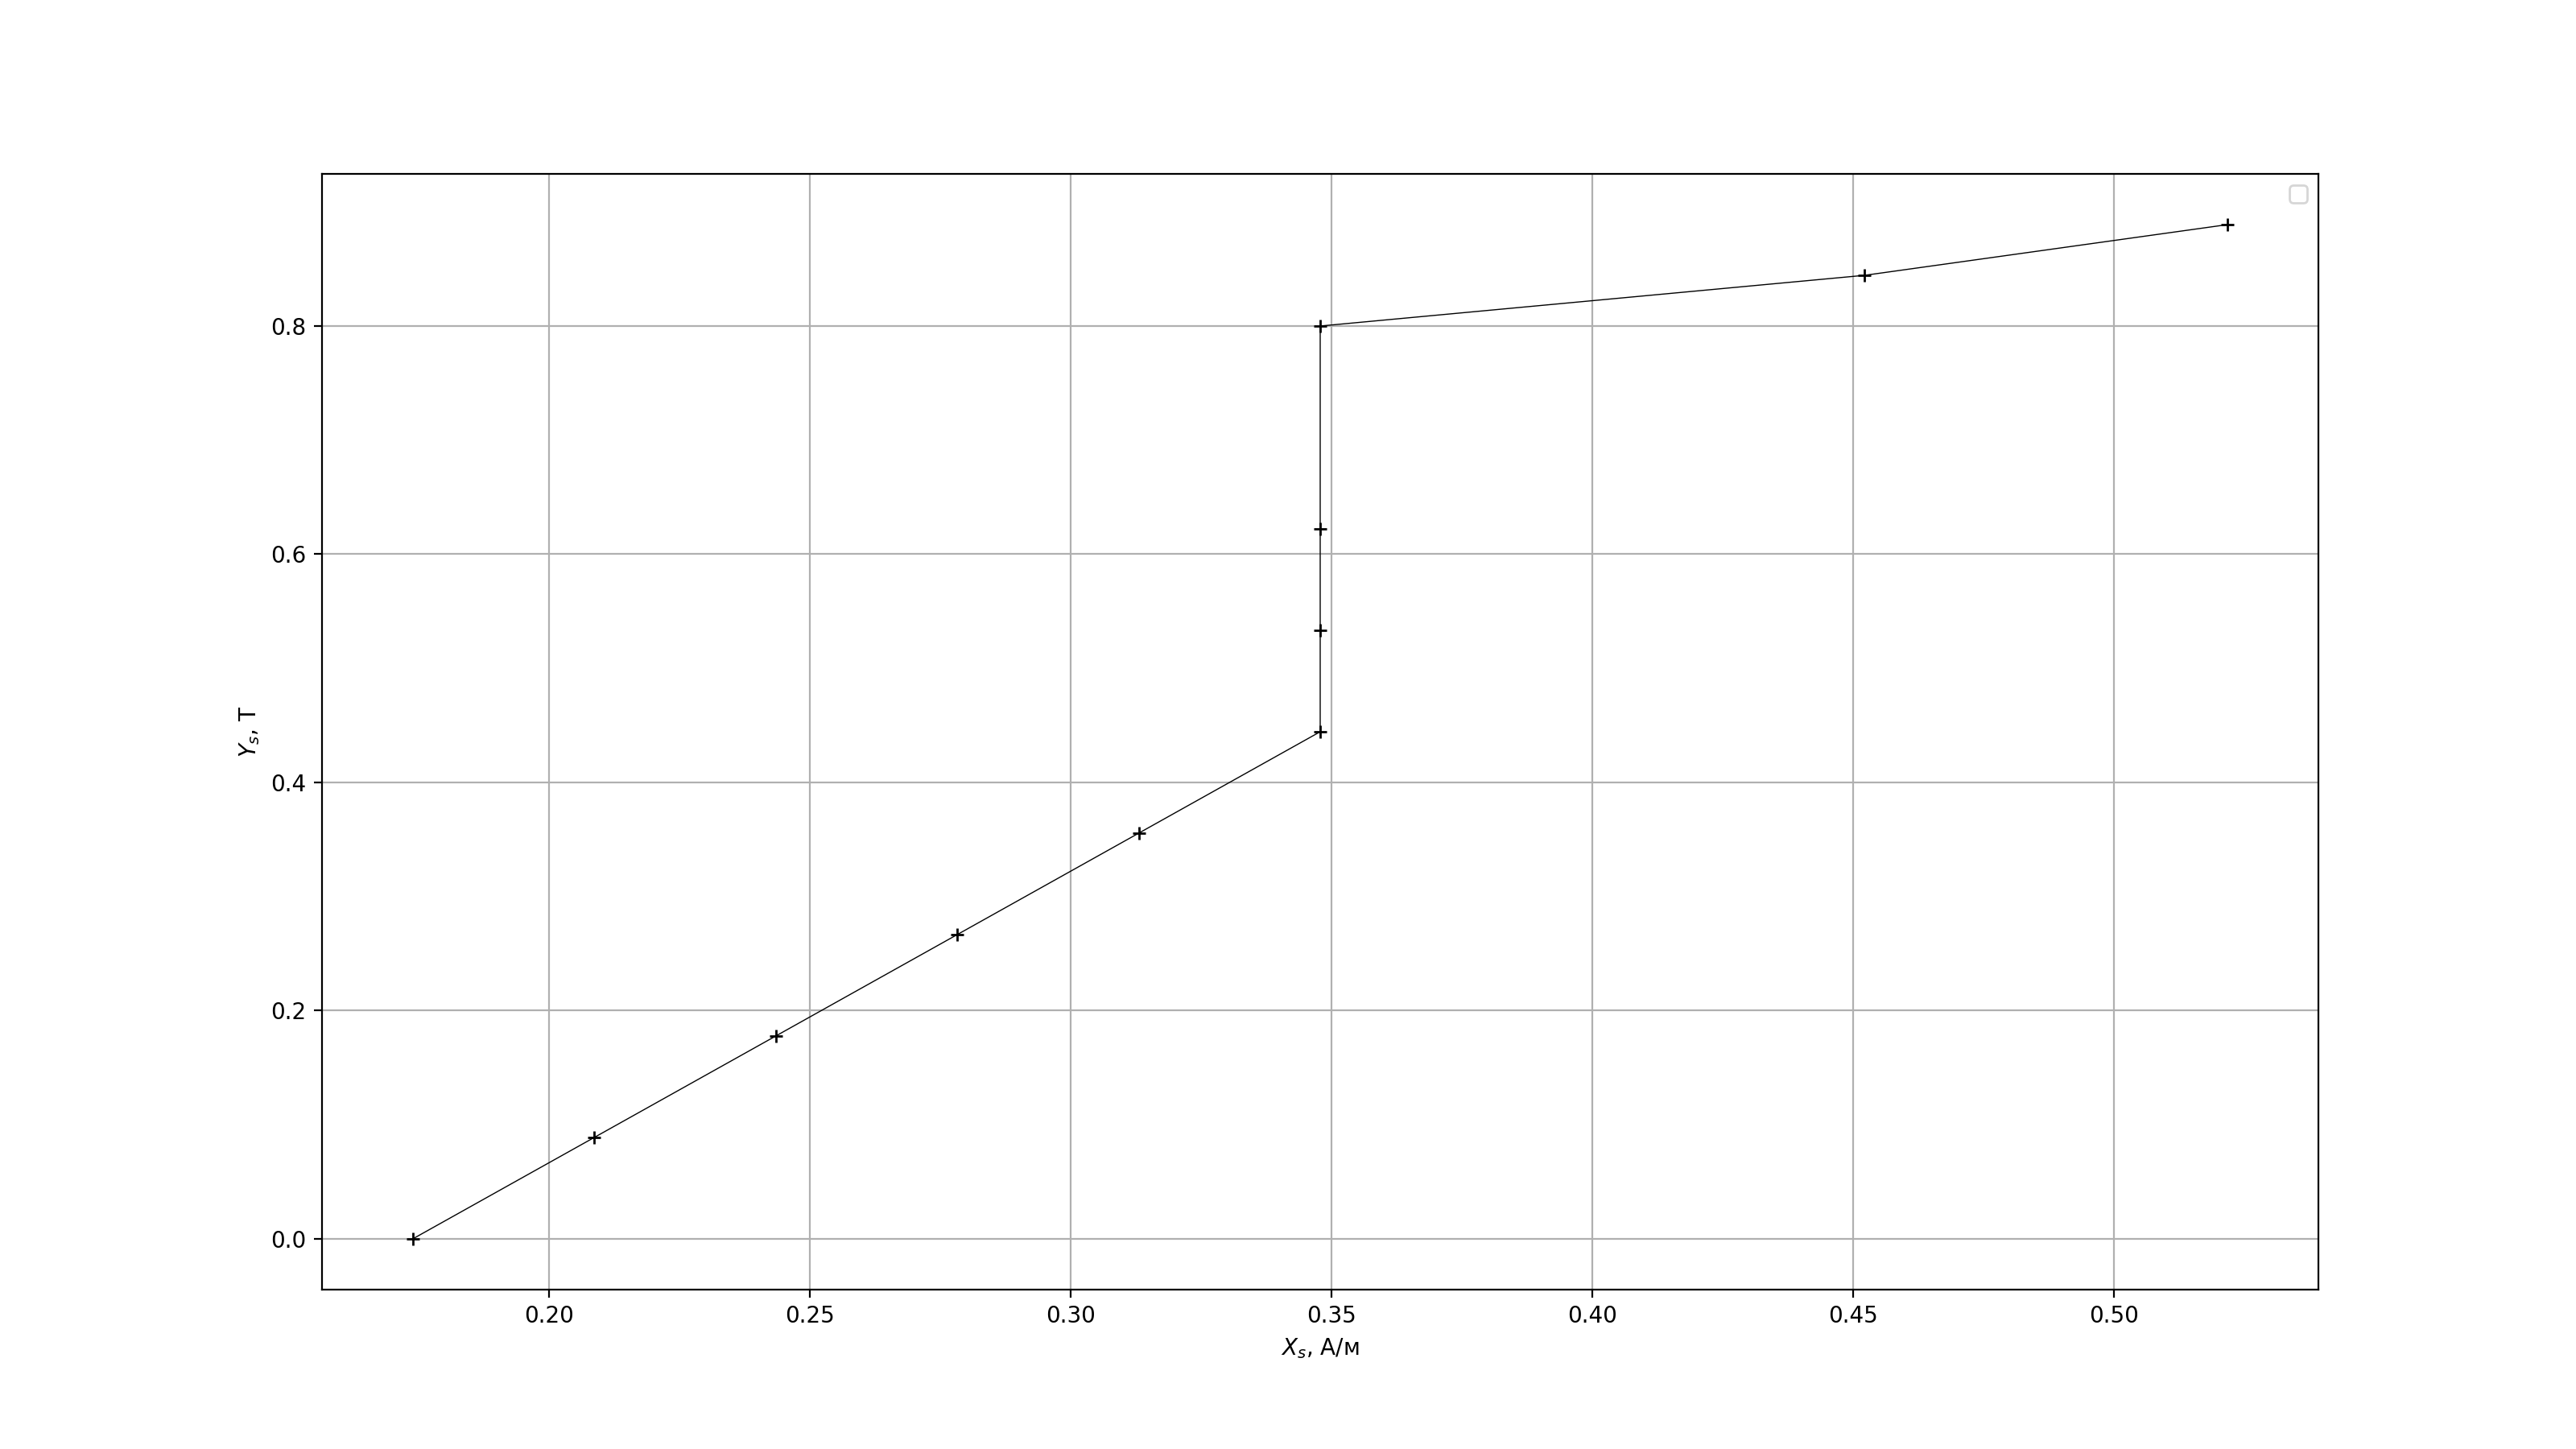
\includegraphics[width=\textwidth]{graph2.png}
            \caption{Начальная кривая намагничивания пермаллоя - график}
        \end{figure}

        \begin{table}[H]
            \caption{Начальная кривая намагничивания феррита}
            \begin{center}
                \begin{tabular}{|c|*{15}{c|}}\hline
                    $x$ & 3.6 & 3 & 2.4 & 2 & 1.6 & 1.4 & 1 & 0.8 & 0.4 & 0.2\\\hline
                    $y$ & 4 & 3.8 & 3.6 & 3.3 & 3 & 2.8 & 2 & 1.6 & 0.8 & 0.4\\\hline
                \end{tabular}
            \end{center}
        \end{table}

        \begin{figure}[H]
            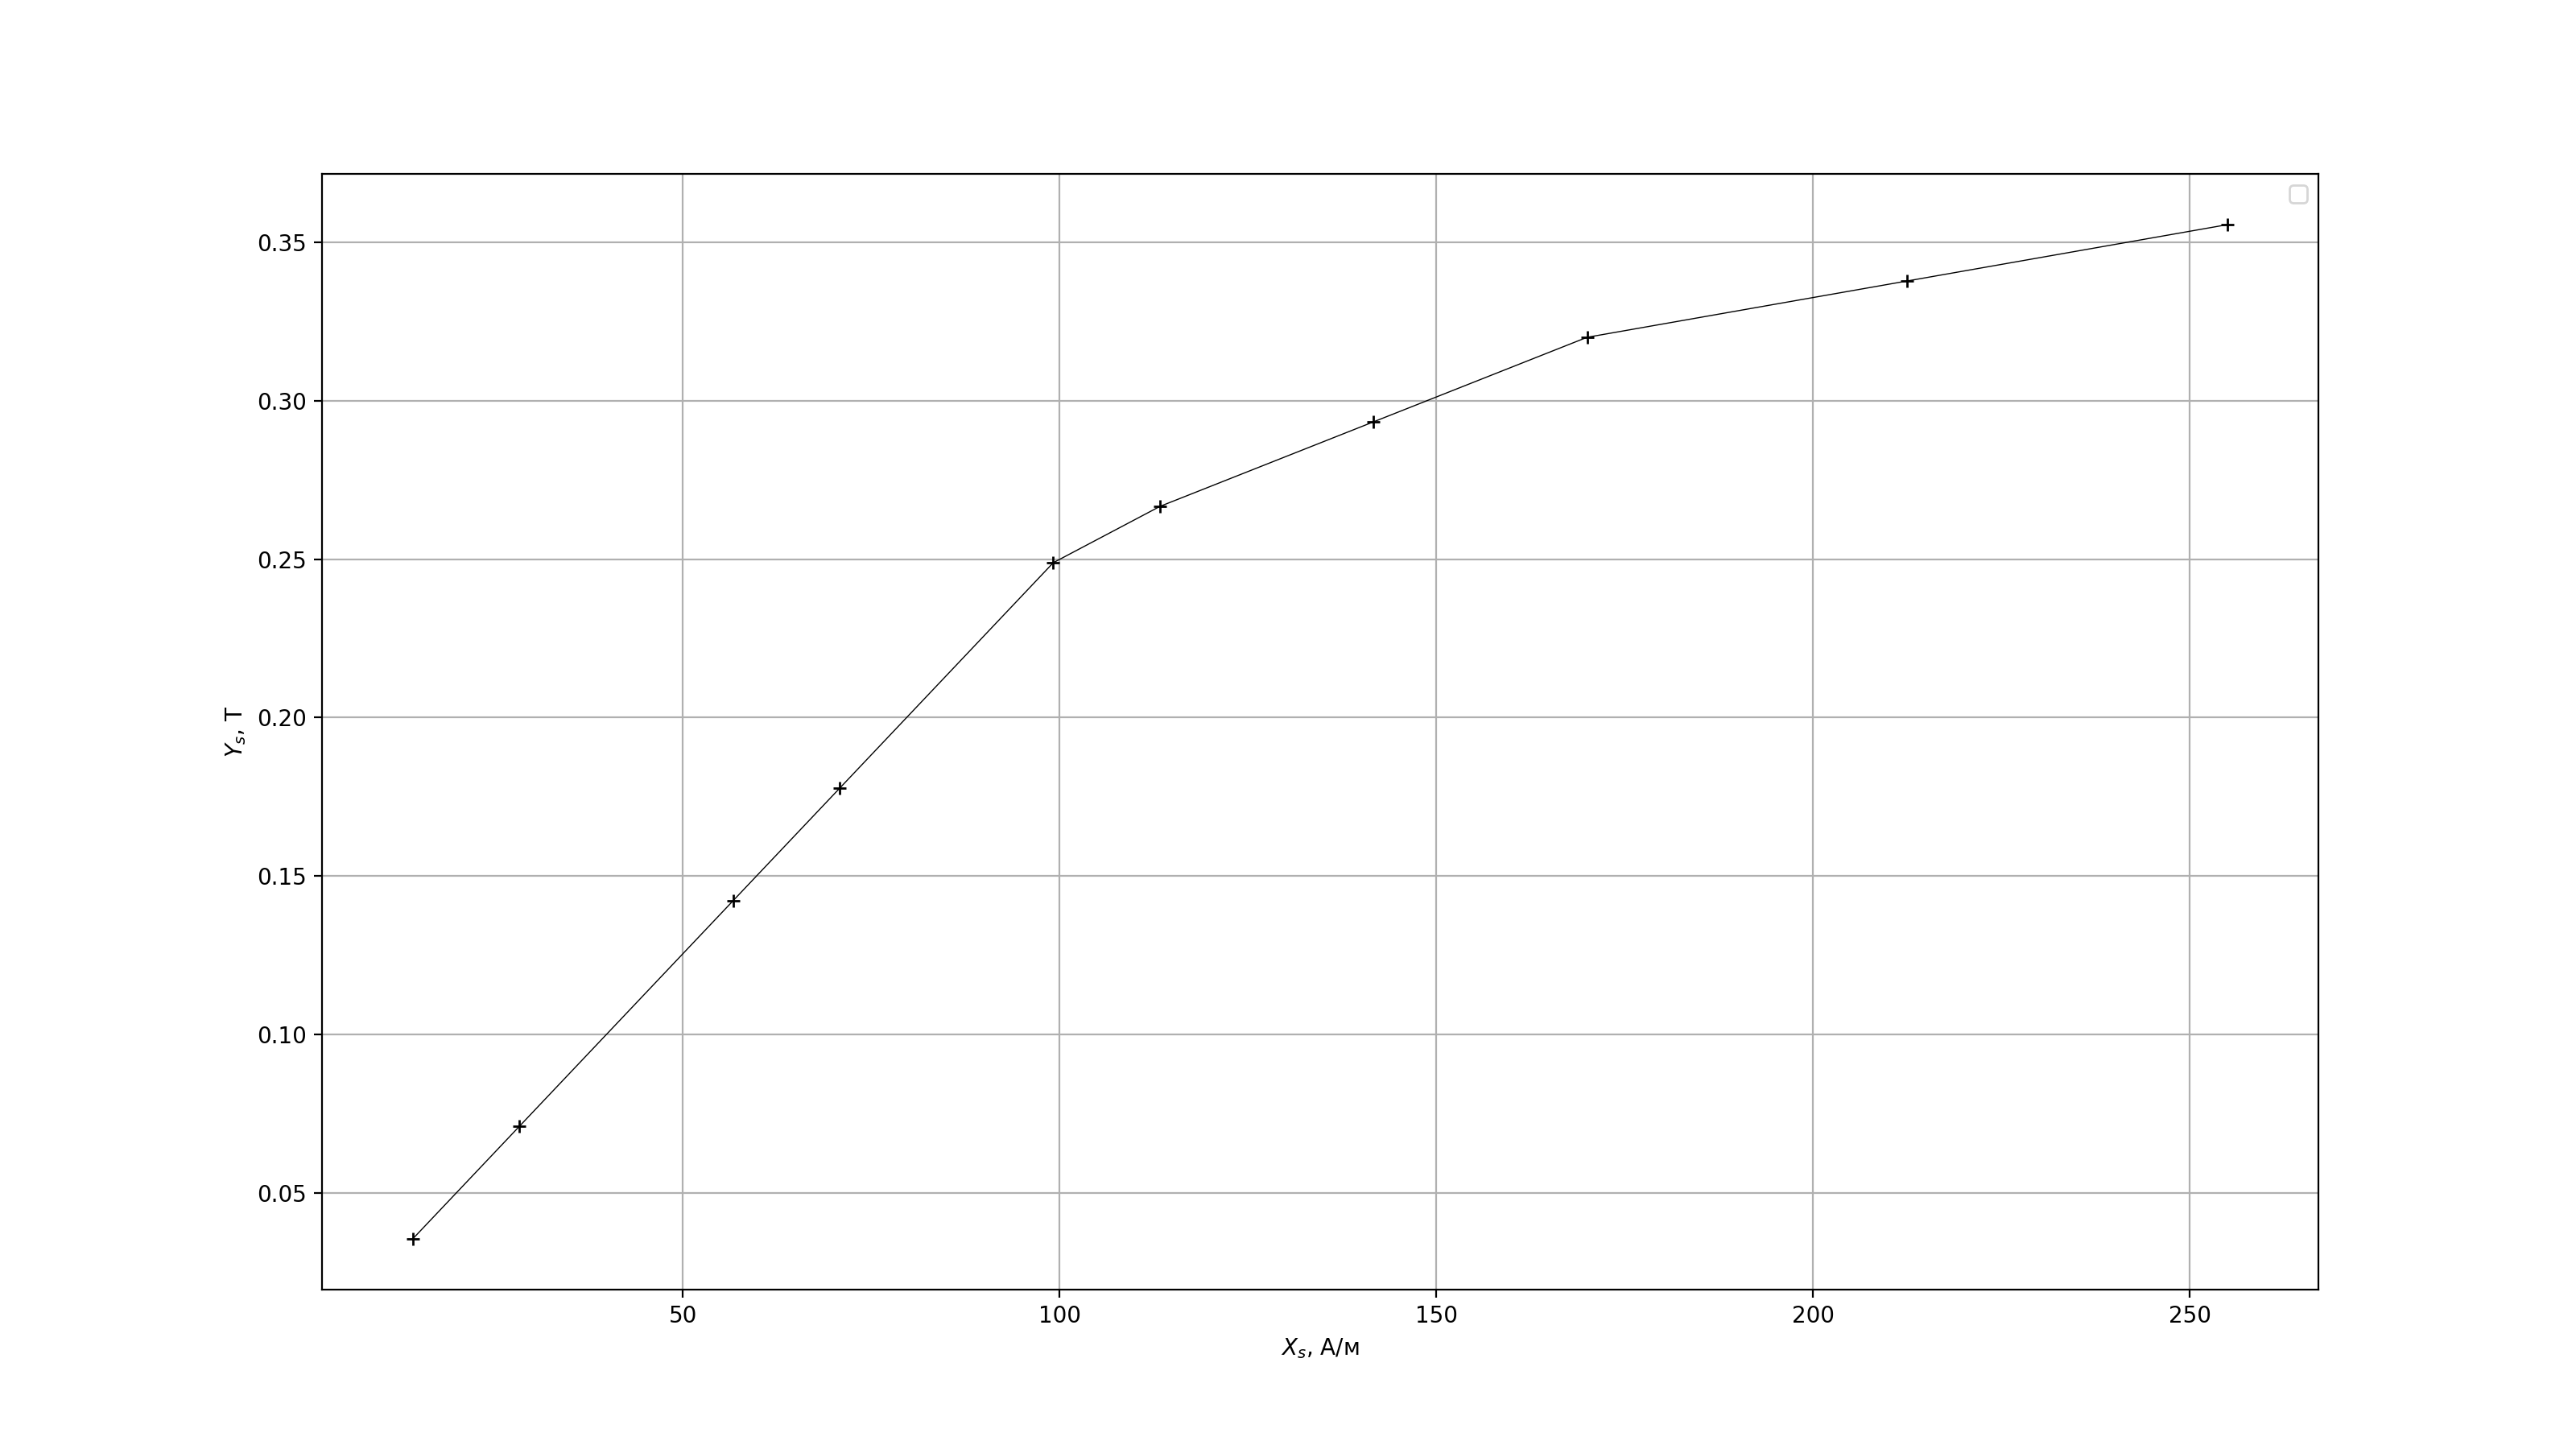
\includegraphics[width=\textwidth]{graph3.png}
            \caption{Начальная кривая намагничивания феррита - график}
        \end{figure}

    \item Восстановим предельные петли для образцов. Рассчитаем  цену
        деления ЭО для петли для оси Х (в $\dfrac{A}{\text{м}}$) по формуле

        $$H=\dfrac{IN_{0}}{2\pi R},$$

        где $I=\dfrac{K_{x}}{R_{0}}$, и в Теслах на деление для оси Y по формуле

        $$B=\dfrac{R_\text{и}C_\text{и}U_\text{out}}{SN_\text{и}}$$

        где $U_\text{out}=K_{y}.$

        \begin{itemize}
            \item \textbf{Кремниевое железо}:

                $H=1.17 \dfrac{\text{А}}{\text{м} \cdot \text{дел}}.$
                $B=0.35 \dfrac{\text{Т}}{\text{дел}}.$

            \item  \textbf{Пермаллой}:

                $H=0.03 \dfrac{\text{А}}{\text{м} \cdot \text{дел}}.$
                $B=0.44 \dfrac{\text{Т}}{\text{дел}}.$

            \item  \textbf{Феррит}:

                $H=1.77 \dfrac{\text{А}}{\text{м} \cdot \text{дел}}.$
                $B=0.22 \dfrac{\text{Т}}{\text{дел}}.$

        \end{itemize}

    \item Соединим вход ячейки с обмоткой "<6.3 В"> трансформатора.

        Определим входное напряжение на $ RC $-цепочке:
        $U_\text{in}=2y\cdot K_{y} = 2 \cdot 8.0 = 16.0$ В.

        Не меняя тока, переключим Y-вход ЭО к выходу ячейки и
        аналогичным образом определим $U_\text{out} = 0.02 * 6.3 = 0.13$ В.

        Определим $\tau = RC $ по формуле

        $$\tau = \dfrac{U_\text{in}}{\omega U_\text{out}} = 0.404 \text{Ом} \cdot \text{Ф}$$

        Найдем $tau_{th}$ - теоретическое значение постоянной времени из параметров RC - цепочки указанных на установке:

        $$\tau_{th} = R \cdot C = 0.400 \text{Ом} \cdot \text{Ф}$$

        Полученные значения достаточно близки чтобы считать их примерно равными (разница в 1\%)

    \item Рассчитаем коэрцитивную силу $H_{c}$ и индукцию насыщения
        $B_{s}$ для каждого образца.

        \begin{itemize}
            \item   \textbf{Кремниевое железо}:

                \fbox{$H_{c}=0.94 \pm 0.07 \ \dfrac{\text{А}}{\text{м}}$}
                \fbox{$B_{s}=0.84 \pm 0.07 \ \text{Тл}$}

            \item  \textbf{Пермаллой}:

                \fbox{$H_{c}=0.63 \pm 0.07 \ \dfrac{\text{А}}{\text{м}}$}
                \fbox{$B_{s}=1.69 \pm 0.07 \ \text{Тл}$}

            \item  \textbf{Феррит}:

                \fbox{$H_{c}=0.71 \pm 0.07 \ \dfrac{\text{А}}{\text{м}}$}
                \fbox{$B_{s}=0.44 \pm 0.07 \ \text{Тл}$}

        \end{itemize}

    \item Из графиков (4-6) оценим максимальные и минимальные относительные значения
        дифференциальной магнитной проницаемости.

        \begin{itemize}
            \item   \textbf{Кремнистое железо}:

                \fbox{$\mu_{min} \simeq 397.11, \, \mu_{max} \simeq 7148.01$}

            \item  \textbf{Пермаллой}:

                \fbox{$\mu_{min} \simeq 3389.41, \, \mu_{max} \simeq 20336.46$}

            \item  \textbf{Феррит}:

                \fbox{$\mu_{min} \simeq 332.87, \, \mu_{max} \simeq 1997.24$}

        \end{itemize}

\end{enumerate}
\end{document}
